\documentclass[main.tex]{subfiles} 
\begin{document}

\subsection{Setup}
This is the experiment we conducted to test the anchoring theory. As described in sections~\ref{anchor} and~\ref{expTheory}, the participants are required to fill out a questionnaire in which they rate the presented features on a scale 1 to 10. This survey starts with a few lead-in questions and then moves on to the features, after the features there is a open text question for feedback and comments and the final question asks the participants to give their overall rating for the eTextbook. The questions display the averages of a 'hypothetical' prior experiment.  

\begin{figure}
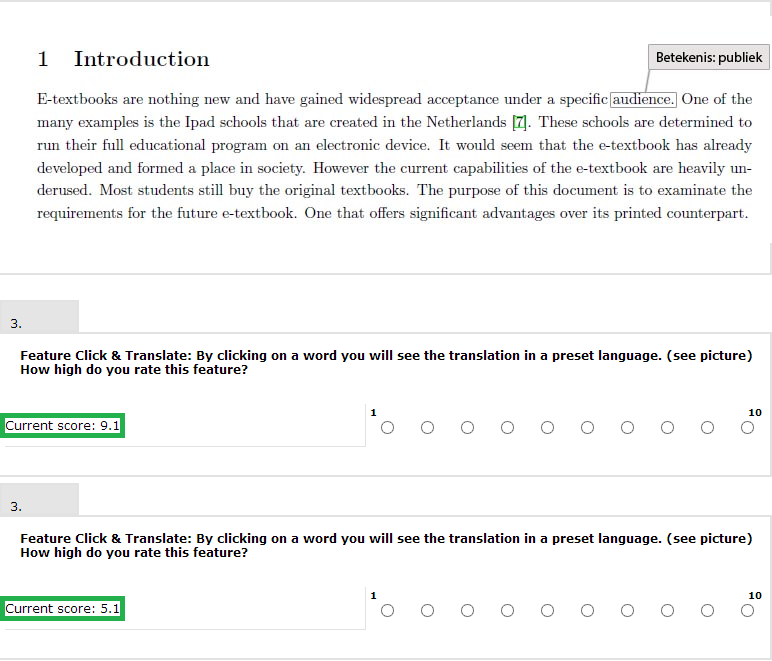
\includegraphics[width=1\textwidth]{QuestionComparison.png}
\caption{The same question, different anchoring point per questionnaire.}
\label{fig:qComp}
\end{figure}

To measure the anchoring effect we created two questionnaires, both using the same questions. While the questions are the same, the averages for the questions are swapped; question `x' is rated high in one and low in the other. This setup can be seen in Figure~\ref{fig:qComp}. After the experiment we measure the average and median of the answers for the high and the low one to see if the anchoring had any effect on our participants.

Our results show that the anchoring effect is obvious in many cases. Only one question has an inconclusive difference and the deviation cannot be contributed to the anchoring effect for sure.

\end{document}
